%!TEX root = ../main.tex
\chapter{2.5维谐振腔的制备与测量} % (fold)
\label{cha:2_5维谐振腔的制备与测量}
	


        \section{器件测量与制备工艺概述} % (fold)
        \label{sec:制备工艺概述}

            由于2.5维谐振腔的电容部分由上下两层金属以及中间的介电层组成,工艺较为复杂,需要至少三步光刻来完成。而细小的电感部分则需要电子束曝光(EBL)来定义形状,再由蒸发镀膜完成。因此,总的制备工艺大致如下:

            \begin{enumerate}
                \item 通过光刻,磁控溅射蒸镀金属Nb,Lift off三步制作平面波导与三层电容的第一层
                \item 通过ALD生长Al$_2$O$_3$,或通过PECVD生长SiO$_2$或SiN$_x$作为电容三层结构中的介电层
                \item 光刻定义掩膜后通过ICP刻蚀或湿法刻蚀介电层
                    \begin{enumerate}
                        \item 显影后剩余光刻胶应完全盖住三层电容的第一层金属以及上方的介电层
                        \item 刻蚀后剩余的介电层仅遮盖住三层电容的底层,其余电介质需被刻蚀以点焊与继续制作其他结构
                        \item 去除介电层上方残存的光刻胶
                    \end{enumerate}
                \item 利用光刻制作出三层电容的顶层图案并蒸镀金属,对准精度约1微米,Lift off
                \item 利用EBL制作微小电感图案
                    \begin{enumerate}
                        \item 电感图案将与三层电容的上下级板相连
                        \item 对准精度 100-1000 nm
                    \end{enumerate}
                \item 旋涂光刻胶,将器件切为4mm~x~7mm大小,清洁器件
                \item 通过点焊将器件与PCB板线路相连接
            \end{enumerate}


            每一步制备工艺的具体步骤与相关参数在附录\ref{cha:fabrication}中给出。
            
        % section 制备工艺概述 (end)


        \section{器件参数设计} % (fold)
        \label{sec:器件参数设计}

            对于LC型谐振腔,其谐振频率为

            \begin{equation}
                \omega_0 = 1/\sqrt{LC}
            \end{equation}
            因此设计器件的关键步骤即为估算其电容值与电感值。

            对于宏观的平板电容,一般的平板电容公式准确性较好,也即
            \begin{equation}
                C = \frac{\epsilon_r \epsilon_0 A }{d}
            \end{equation}
            其中$A$为平行板的面积,$d$为平行板的间距,也即介电层的厚度,$\epsilon_r $为介电层的相对介电常数。通过查询,可得可能选用的介电材料的相对介电常数\cite{cardarelli2008materials},如表所示。


\begin{table}[htb]
  \centering
  \caption{可能用到的介电材料的相对介电常数\cite{cardarelli2008materials}}
  \label{tab:dielectricConstants}
    \begin{tabular}{c|ccc} %{\linewidth}{lX}
      \toprule %[1.5pt]
      介电材料& Al$_2$O$_3$ & SiO$_2$ & SiN$_x$ \\
      \midrule %[1pt]
      $\epsilon_r $ & $9.0$ & $3.79\sim 4.5$ & $ 7.9\sim 8.1 $  \\
      \bottomrule %[1.5pt]
    \end{tabular}
\end{table}
            
            对于电感的估计,可以采用COMSOL仿真与经验公式计算这两种方法,但均有较大误差。COMSOL仿真所得出的电感明显依赖于仿真空间区域的大小,见第\ref{sub:电感设计与优化}节中的分析。而对于利用经验公式\ref{eqn:SelfInductance}估计电感,对于实际中有几何形状的电感也将给出有所偏差的电感值。综合这些考虑,对电感的估计能够达到的精度限于数量级的程度。因此,我们最终设计的器件频率变化范围较大,从而能够容忍估算中带来的误差。由于对电容的估计较为准确,我们可以通过一组变化电容大小,固定电感的谐振腔,通过测量频率,即可反解或拟合出电感值的大小。利用相同的思路,也可通过一组变化电感大小,固定电容的谐振腔,进一步确定对于电容的计算是否准确。最终,我们设计了四组测试器件,两组固定两个不同的电容值,对电感值有一系列变化,另两组固定两个不同的电感,对电容的大小进行一系列变化,可参阅第\ref{sec:光刻板的设计}节的光刻板图案。设计所用的尺寸与估计的对应频率见表所示。
            
            
        % section 器件参数设计 (end)




        \section{光刻板的设计与改进} % (fold)
        \label{sec:光刻板的设计}

            由于制备工艺需要三步光刻,对于完整制备一个器件来说,需要的光刻板的图案为一组三个,分别对应\ref{sec:制备工艺概述}制备工艺概述中的前三步。第一步完成二维平面波导以及接地平面的制作,以及三维电容的第一层金属。第二步在生长介电材料后通过光刻制作掩膜覆盖住需要保留的电容的第二层介电层部分,并刻蚀掉没有被覆盖掉的电介质。第三部制作出电容最上层的金属。最后一步通过电子束曝光与蒸镀制作微小的电感部分,并各自与三维电容的上、下两层连接起来。光刻的三个步骤所需的模板作图如图\ref{fig:one_group}所示
            

            \begin{figure}[h]
                \centering
                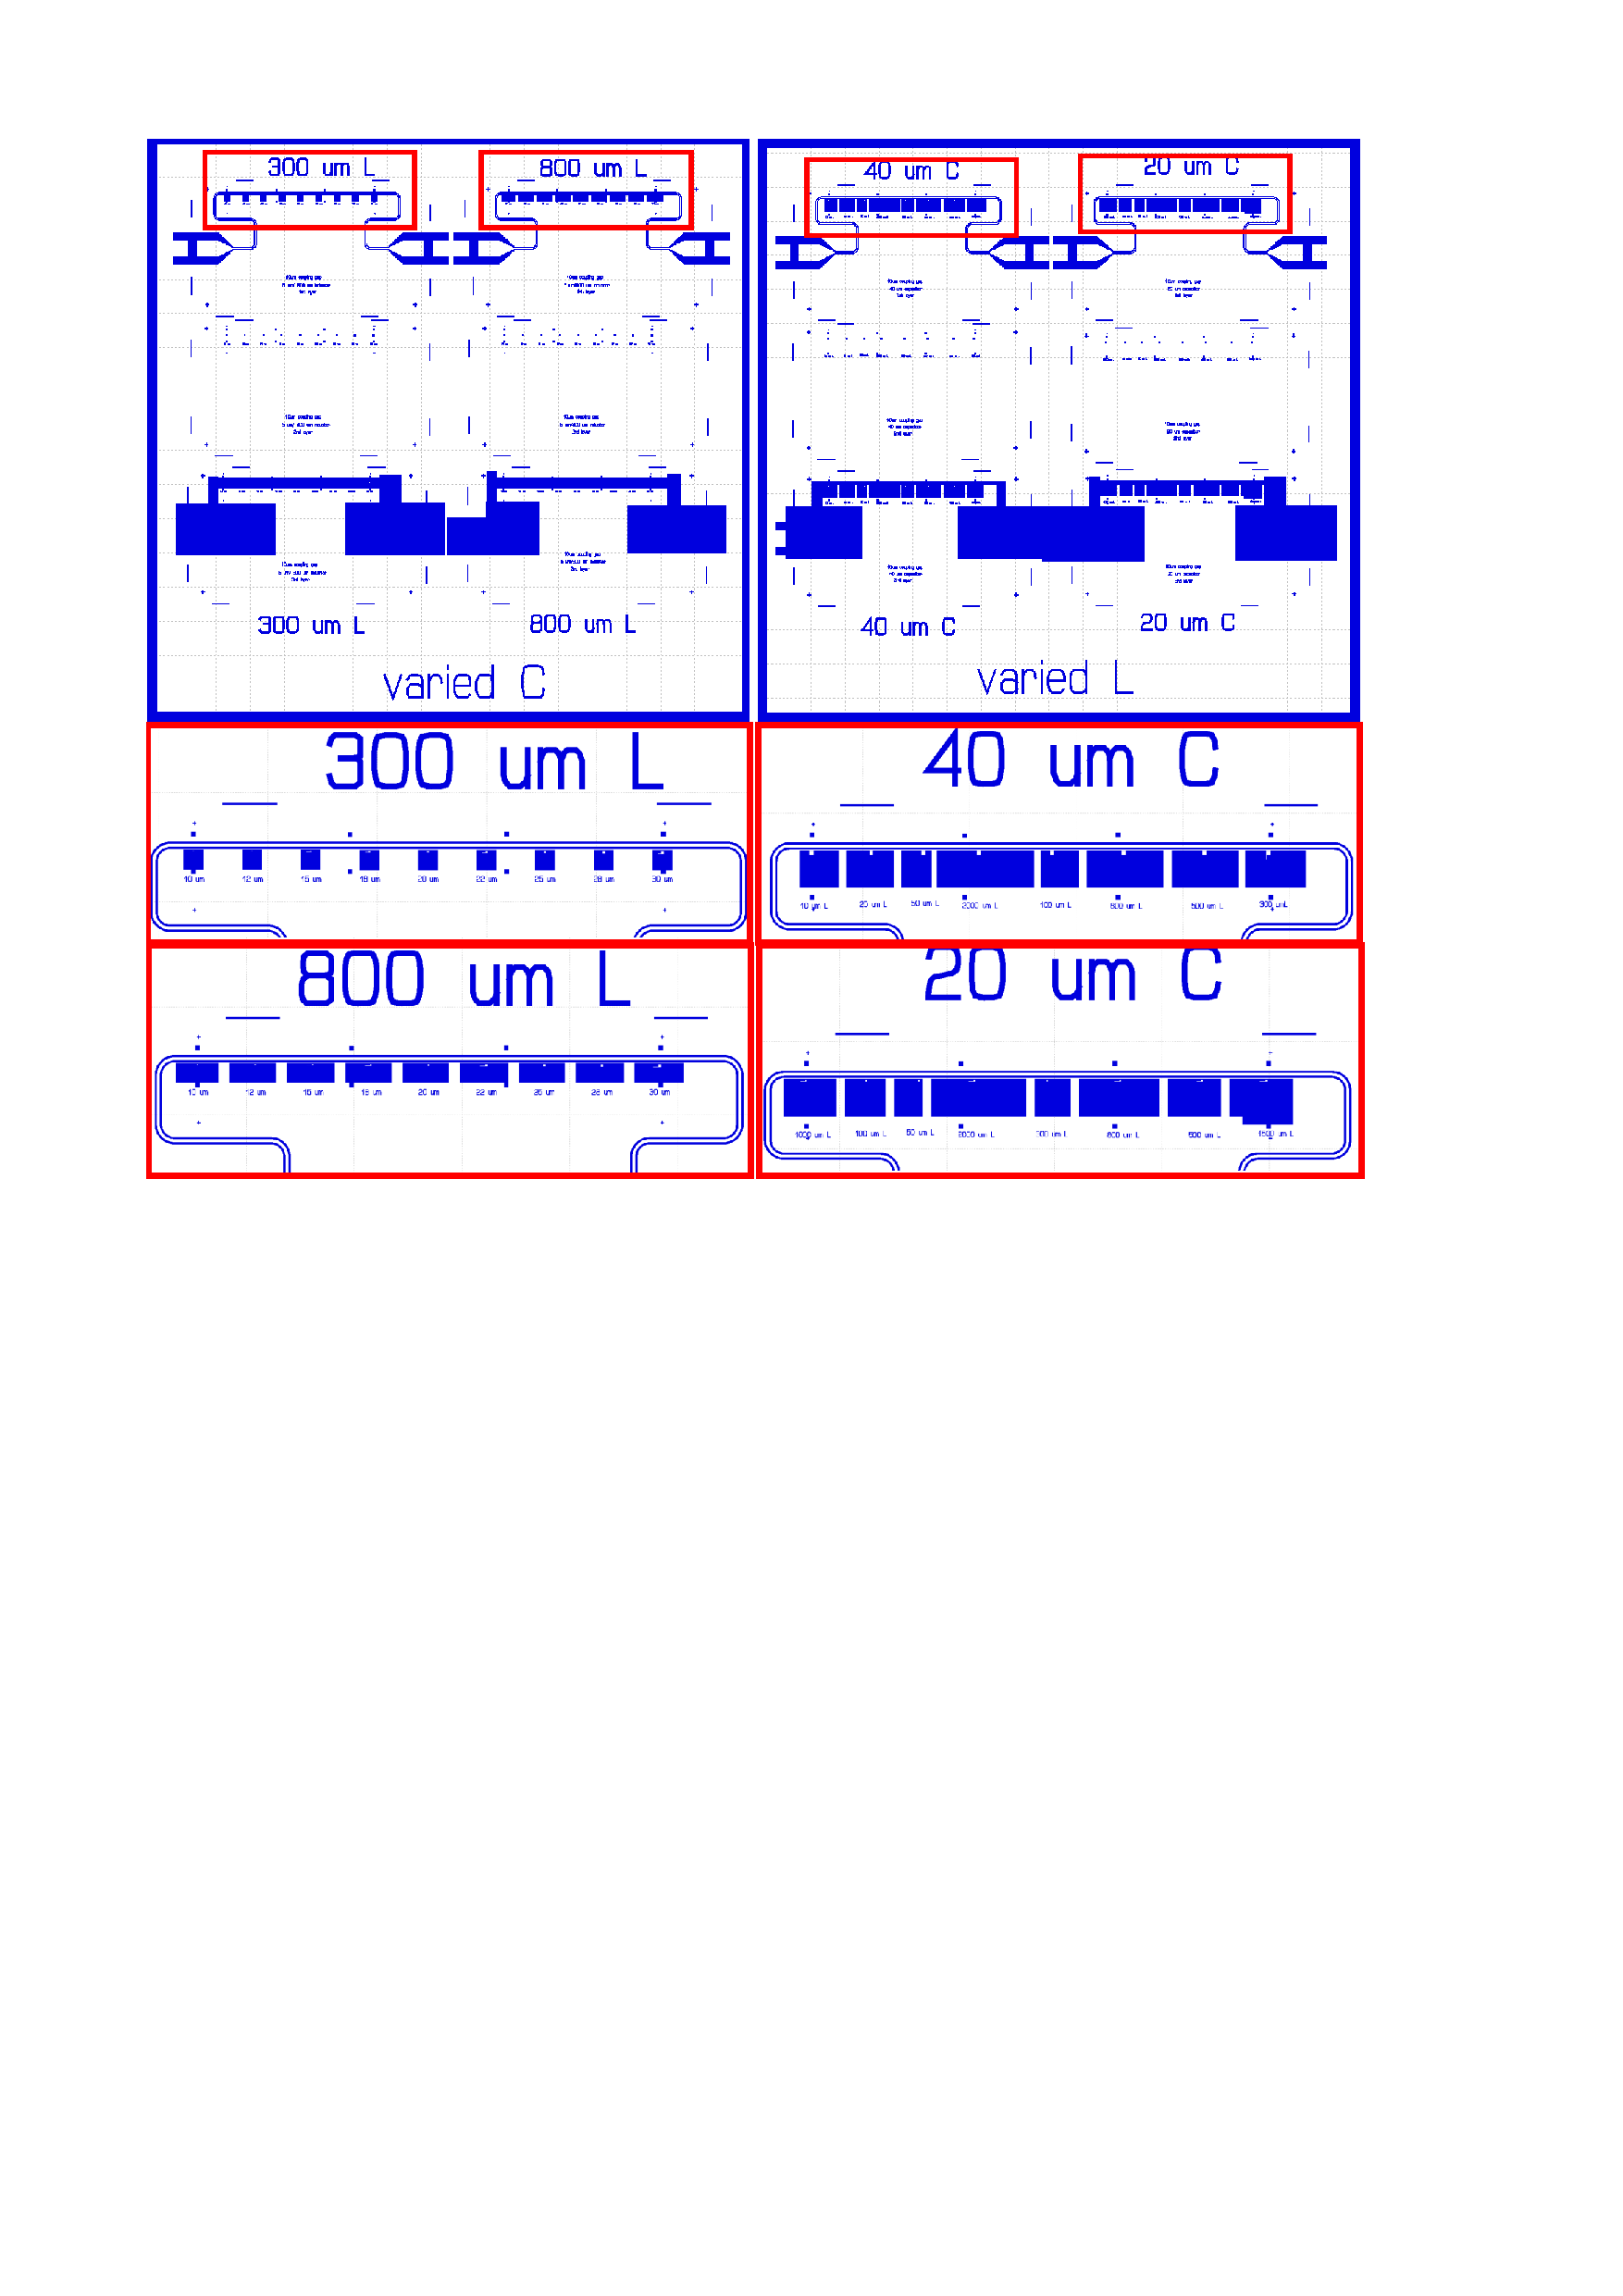
\includegraphics[width=\textwidth]{PhotoMaskTest.pdf}
                \caption{制备一个器件所需的三个光刻步骤对应的一组三个模板图案}
                \label{fig:one_group}
            \end{figure}

            \begin{figure}[h]
                \centering
                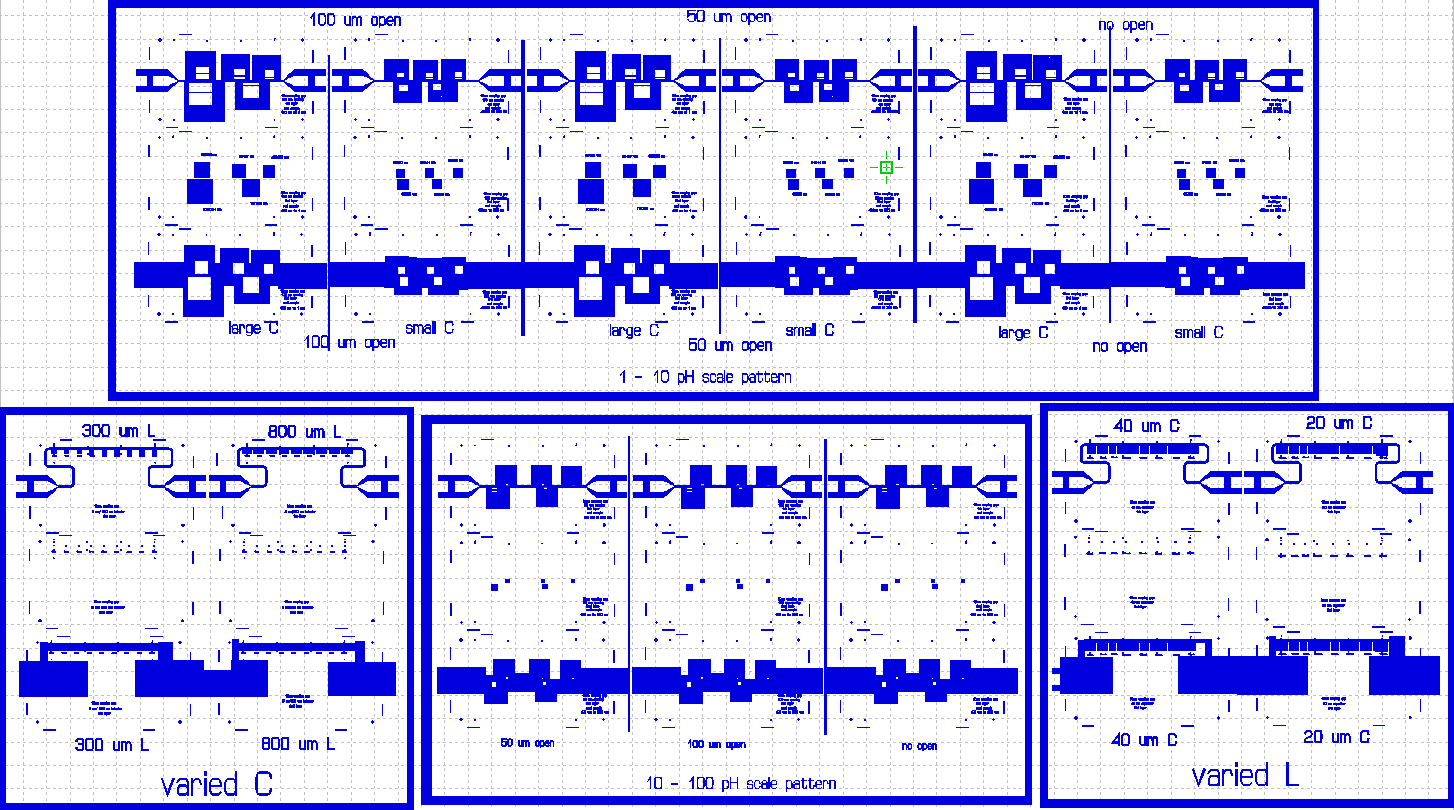
\includegraphics[width=5in]{fab/PhotoMaskAll.png}
                \caption{完整的光刻板图案}
                \label{fig:LC}
            \end{figure}

            由于没有这类谐振腔的制备经验,对于其频率的估算并没有太多把握,因此我们希望有尽可能多的谐振频率与设计相对应的数据,来辅助下一步对仿真结果的修正与器件制备的改进。由于对电容和电感估值的准确度均有待确认,我们需要至少两组不同的器件设计的组合,一组固定$L$变化$C$的大小,另一组固定$C$变化$L$的大小,这样可以通过拟合确定出每个器件的$L$与$C$的值。因此,一个二维平面波导可以与多个谐振腔耦合,可方便测量。另一方面,考虑到电子束曝光难度与耗时均较大,我们打算先尝试中等数值的电容与电感组合,使电感的尺寸能够通过光刻制备,这样即可在三层电容制备的最后一步同时制作出电感,省去了电子束曝光制备电感的步骤,大大加快样品制备与测试速度。解决三层电容的制备后,再通过电子束曝光制作电感。

            综合上述讨论,我们总共设计了若干种不同的模板几何形状,如图\ref{fig:LC}所示,覆盖了较大范围的电容与电感值,为第一次摸索器件制备工艺以及尝试性测量提供较大的频率变化区间,尽可能保证能够测到谐振腔的共振频率。





            \section{器件制备情况与改进} % (fold)
            \label{sec:器件制备情况与改进}
                按照上述计划,我进行了器件制备的工作,目前已完成了两轮完整的器件制备流程。

                在第一轮器件制备过程中,发现了许多问题,并依次进行了分析与解决。第一轮器件制备的器件图像如图\ref{fig:FabRound1}所示,均为通过显微镜拍摄的器件实物图。

            \begin{figure}[h]
                \centering
                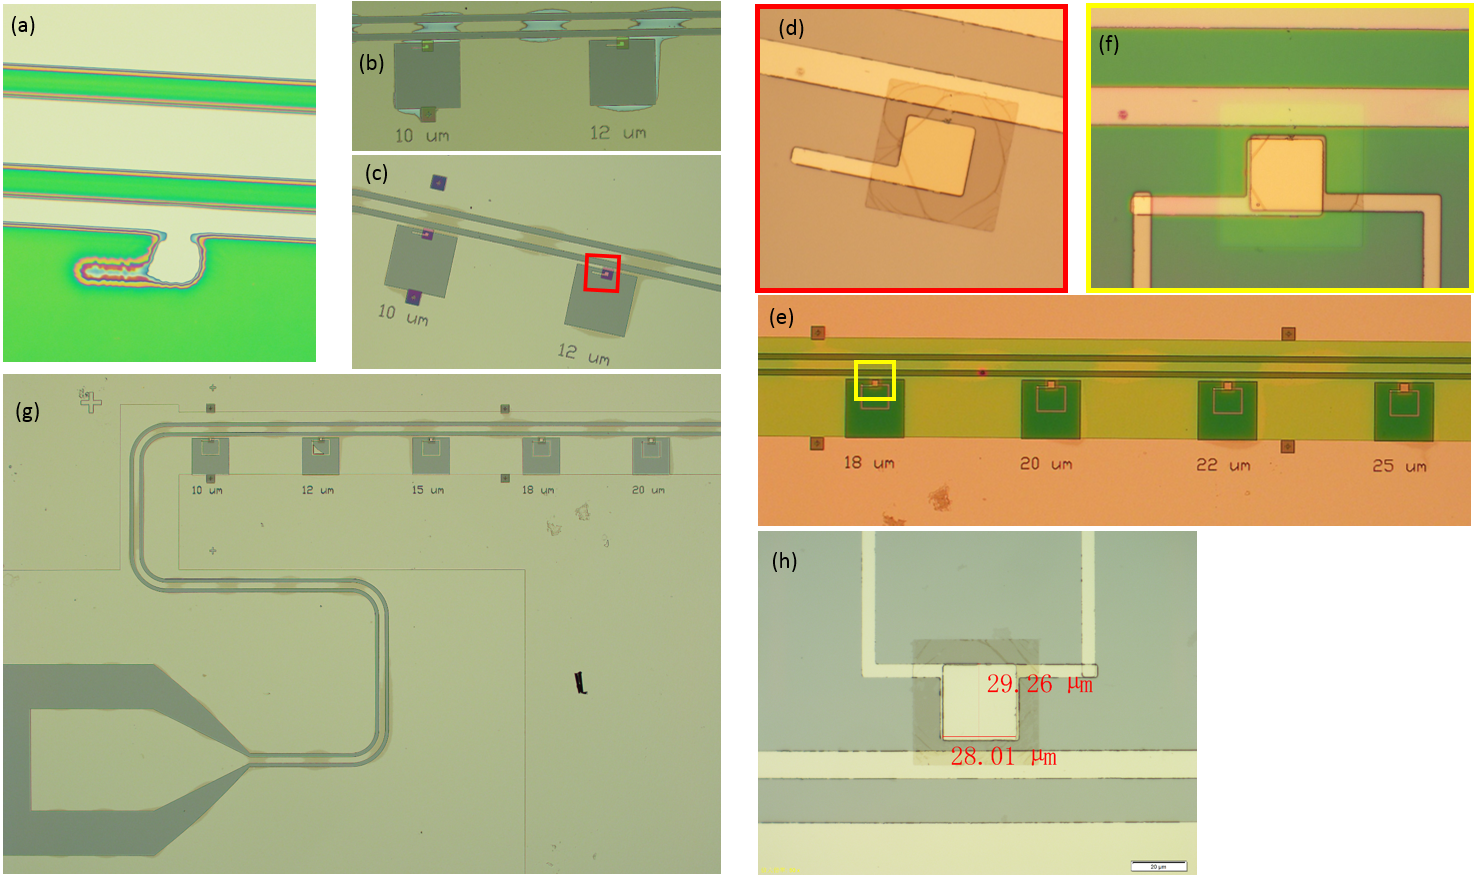
\includegraphics[width=\textwidth]{FabRound1.png}
                \caption{第一轮器件制备过程}
                \label{fig:FabRound1}
            \end{figure}

            由于PPMS测量系统仅可放下大小为4mm~x~7mm的器件,我们最初即采用该大小的硅片作为衬底开始进行微纳加工。由于器件尺寸较小,在旋涂光刻胶的过程中导致胶厚分布不均,因此光刻第一层图案后效果明显不好,如图\ref{fig:FabRound1}(a)所示。图\ref{fig:FabRound1}(a)中绿色部分为显影后剩余的光刻胶,也即不会被蒸镀上金属的部分。靠上的两个长条形的绿色部分即为平面波导的中心线与两侧接地部分间的间隙,而下面大块绿色部分包围着的即应该为三维电容结构的三层中的第一层。由于光刻胶厚度不均匀,曝光过程中发生了衍射,导致图案变形。因此,我们改用8mm~x~8mm左右大小的硅片进行微纳加工,再在最后点焊前将器件切割为PPMS所要求的大小。进行这步改进后,光刻效果很好,器件的第一层金属顺利完成,对应第\ref{sec:制备工艺概述}节中的步骤1。

            器件制备的第二步,也即生长介电层的步骤较为简单,利用超净间内现有的PECVD或ALD的相关程序即可自动完成。第一轮器件制备选用的介电层为PECVD生长的30nm的SiO$_2$。在进行第三步,也即第二层光刻的显影阶段时,我观察到了器件上有淡蓝色的杂物,疑似为未清洗干净的被曝光的光刻胶,如图\ref{fig:FabRound1}(b)所示,其中浅绿色的小方块即为理应存在剩余光刻胶的部分,成功观察到了完整盖住三维电容第一层金属以及上方介电层的光刻胶。分析后我们认为,残存的光刻胶可能导致该处剩余未被刻蚀的介电层,对器件不会产生本质影响,因此我们暂时忽略这一步的不理想,继续器件制备。进行ICP刻蚀后,器件如图\ref{fig:FabRound1}(c)所示,可以看见电容处的电介质与残留的光刻胶整体呈现深紫色,而图\ref{fig:FabRound1}(b)中的淡蓝色部分仍旧为灰色阴影,应为未刻蚀干净的介电层。图\ref{fig:FabRound1}(c)中还能看到其他两块紫色区域,为第二层光刻对准第一层结构所用的标记符号,因为也没被曝光所以留下了介电层与光刻胶,从而呈紫色。在最后去除介电层上方残留光刻胶时,使用了常用的S1805光刻胶去胶液NMP,但去胶后观察到了剩余的介电层表面有不明灰色纹路,如图\ref{fig:FabRound1}(d)所示。图\ref{fig:FabRound1}(d)即图图\ref{fig:FabRound1}(c)中红色矩形部分去胶后的放大图。这些灰色纹路疑似为未被去净的光刻胶,因此在第二轮器件制备过程中,我们改用PG remover去胶,得到了更好的效果。

            第二、三步完成后,进行最后一步的制作电容的顶层金属。首先进行顶层图案的光刻,光刻的效果如图\ref{fig:FabRound1}(e)与(f)所示,其(f)为(e)中黄色矩形的放大图。可以看出,顶层与底层间有一定的对准误差。需要注意,在将电感部分与顶层金属和底层金属连接上时,需先通过Argon milling去除底层金属表面的氧化层,随后磁控溅射Nb,才能达到良好的电接触。蒸镀完成后,即可去胶使设计的金属结构存留。此时因为与上下两层电容金属极板相连的电感在平面内围成闭合区域,去胶液难以进入。正常情况下可以尝试超声,但目前器件上有较薄的介电层,容易在超声过程中脱落,因此我们小心尝试了超声的功率与持续时间,最终在保持介电层完整的条件下达到了较好的去胶效果,如图\ref{fig:FabRound1}(g)所示。可以看到,绝大部分应被去掉的金属均成功被去掉,除了第二个谐振腔中电感部分的左下角内仍有一小块金属。

            至此,器件制备基本结束,制备出的2.5维谐振腔如图\ref{fig:FabRound1}(h)所示,电容的下层与上层极板间的对准误差大概在1um,与预期相符。灰色方形部分为上下极板间的介电层,细条形为电感。最后旋涂光刻胶,切片并清洗后,即可进行点焊,并放入PPMS进行测量。第一批器件的测量结果在第\ref{sec:2.5维谐振腔的测量与讨论}节中进行了分析与讨论。


            第二批器件的制备过程如图\ref{fig:FabRound2}所示。



            \begin{figure}[h]
                \centering
                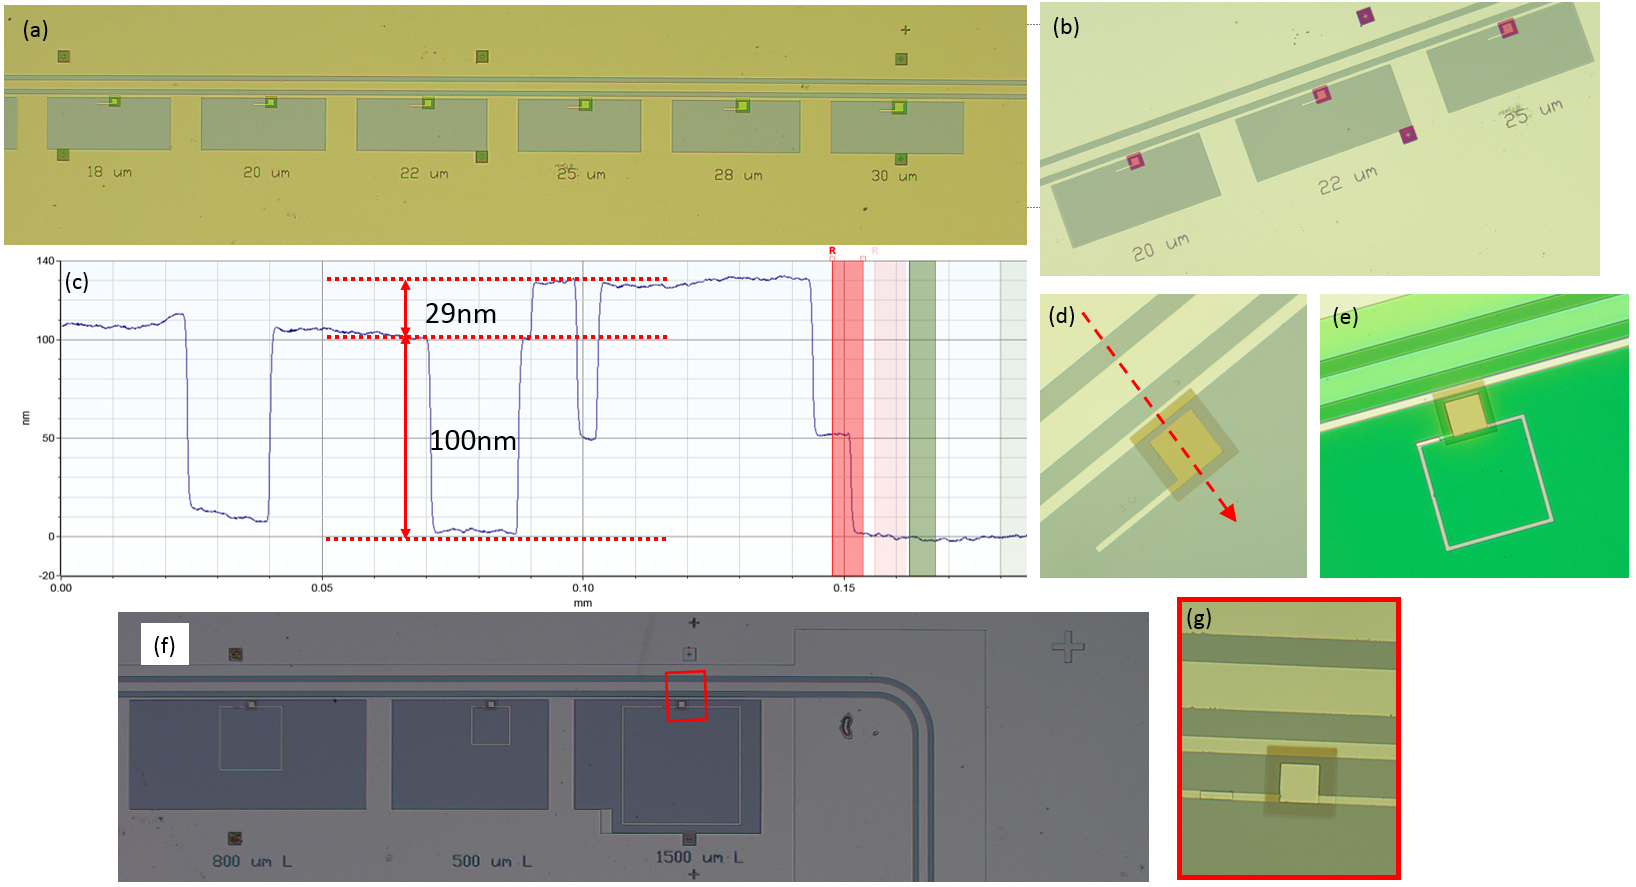
\includegraphics[width=\textwidth]{FabRound2.png}
                \caption{第二轮器件制备过程}
                \label{fig:FabRound2}
            \end{figure}

            经过第一轮器件制备的问题与经验后,第二轮器件制备效果有很多改善。考虑到SiN$_x$与SiO$_2$相比介电常数更高(见表\ref{tab:dielectricConstants}),能够得到相对更高的电容,从而导致谐振频率更低,使更多器件进入测量系统的测量范围,第二轮器件的介电层采用SiN$_x$制作。图\ref{fig:FabRound2}(a)为第一层金属制备并生长介电层后通过光刻定义刻蚀介电层的掩膜,图中淡黄色部分为蒸镀的第一层Nb金属区域以及上方覆盖的介电层,淡墨绿色部分为硅衬底加上覆盖的介电层,若干亮绿色的小方块则为显影后剩余的光刻胶。可以看出,前两次的光刻效果均很好。ICP刻蚀介电层后的器件图如\ref{fig:FabRound2}(b)所示,介电层被刻蚀后第一层金属的颜色更加明亮,与第一轮器件制备中观察到的现象相同,见图\ref{fig:FabRound1}(b)与图\ref{fig:FabRound1}(c)。被ICP刻蚀后的光刻胶与介电层部分变为紫红色,与图\ref{fig:FabRound1}(c)类似。由于第一轮器件制备使用NMP去胶液后发现介电材料上有残余灰色纹路,疑似残留的光刻胶,于是我们改用PG Remover去胶,详细流程可参考附录\ref{cha:fabrication}。去胶后的器件如图\ref{fig:FabRound2}(d)所示,介电层表面平整,无可见的残留物。我们沿图\ref{fig:FabRound2}(d)中红色箭头轨迹测量了样品表面高度的变化,结果如图\ref{fig:FabRound2}(c)所示。红色箭头首先跨越平面波导传输线,后经过位于第一层金属表面上的介电层,位于硅衬底上的介电层,位于第一层电容金属极板上方的介电层,位于硅衬底上的介电层,最后回到衬底表面。从该截面处样品表面距衬底的高度变化能明显看出所生长的第一层金属层厚度约为100nm,第二层介电层厚度约为29nm,均与设计相符。值得注意的是,直接与衬底接触的介电层厚度为约50nm,我们猜测原因可能为PECVD生长速率与衬底类型有关,尚待进一步确认。

            完成第三层的光刻显影后,器件图如图\ref{fig:FabRound2}(e)所示,能看出光刻本身与对准状况均良好。采用摸索出的lift off超声方法,在保证介电层完整的条件下去除不要的金属区域,最终效果如图\ref{fig:FabRound2}(f)与(g)所示,在23个LC谐振腔中,仅有一个lift off未能成功。完成微纳加工后的器件,旋涂光刻胶,切片并清洗后,即可点焊并放置入PPMS中进行测量。



            % section 器件制备 (end)
            



            \section{2.5维谐振腔的测量与讨论} % (fold)
            \label{sec:2.5维谐振腔的测量与讨论}
            	

            我首先对器件进行了频率扫描,观察到了若干较宽的谐振峰,疑似为2.5维谐振腔的模式,但与设计所对应的相比耦合偏强且$Q_i$偏低。于是我进一步在不同磁场下测量了频率响应,结果如图\ref{fig:LC_R1_meas}所示。


            \begin{figure}[h]
                \centering
                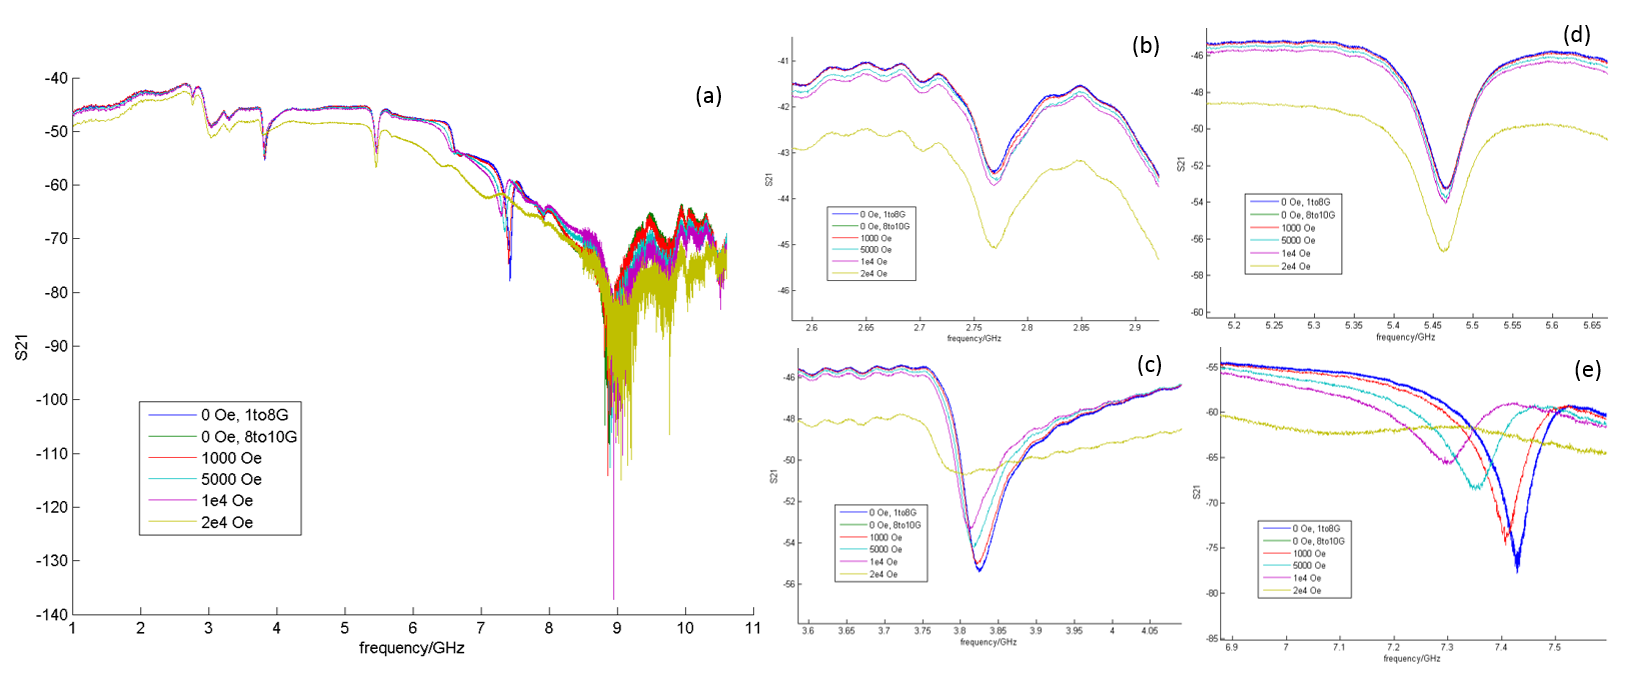
\includegraphics[width=\textwidth]{LC_R1_meas.png}
                \caption{第一批2.5维谐振腔器件的测量结果}
                \label{fig:LC_R1_meas}
            \end{figure}


            通过图\ref{fig:LC_R1_meas}我们观察到了四个疑似的谐振模式,通过拟合得到的品质因子均在100的数量级,与通常的谐振腔品质因子相比低了两三个数量级。图中不同颜色的曲线代表不同磁场下的频率响应,磁场的单位为高斯。图\ref{fig:LC_R1_meas}(b)至(e)为图\ref{fig:LC_R1_meas}(a)中四个疑似谐振模式频率附近的放大图。通过不同磁场下的曲线能明显看图\ref{fig:LC_R1_meas}(b)与(d)中的模式随磁场变化很小,仅为整体高度的平移,而图\ref{fig:LC_R1_meas}(c)与(e)的模式峰形随磁场变化明显。由此可知,图\ref{fig:LC_R1_meas}(c)与(e)的模式与器件相关,在器件处于较强磁场下性质变差后也发生明显变化,而图\ref{fig:LC_R1_meas}(b)与(d)的模式则可能为样品盒的模式,随磁场变化不明显。


            我们分析后认为图\ref{fig:LC_R1_meas}(c)与(e)的模式是否为所设计的2.5维谐振腔的模式还有待进一步验证,所观察到的随磁场变化的峰可能为与超导性质相关的谐振模式,不一定为所设计的谐振腔。

            对于器件可能出现的问题以及未观察到可靠信号的原因,我们大概分析了以下三点以及相应的改进方案:
            \begin{enumerate}
                \item 电容的底层与顶层是否成功通过电感导通以保证器件制备的正常:通过器件制备过程中同时制备陪片使电容上中下三层错开,制备结束后可直接用Probe station测量电阻大小,进而判断导通情况
                \item 器件的频率估计准确度较差,能否保证有器件位于PPMS测量系统的频率范围内:使用器件频率变化范围更宽的设计
                \item 器件与CPW的耦合较弱,导致信号较小,被噪声覆盖:使用耦合更强的设计,如插指型电容耦合\cite{goppl2008coplanar}
            \end{enumerate}

            综合上述讨论,第一轮器件制备测量结果不理想原因主要有以下两方面:一方面,由于介电材料相对于空气而言有损耗,谐振腔的$Q_i$比常见传输线谐振腔更小,而由于光刻板的设计使谐振腔与传输线中的场间有一段距离的接地平面,有一定屏蔽作用,导致谐振腔与传输线中的模式耦合较弱,$Q_c$较大,综合这两点,预计谐振腔响应的峰形较浅较宽,可能被背景噪声覆盖;另一方面,器件制备过程中最上层与最下层的对齐误差导致电容偏小,谐振腔频率偏高,可能使谐振频率超出PPMS与VNA测量系统的正常测量范围$1\sim 10$GHz。因此,我们下一步改良了光刻板的设计,增大谐振腔与传输线的耦合强度从而增强谐振腔响应的信号。同时开始第二批器件的制备,采用谐振频率变化范围更广的器件组以使得有谐振腔的频率落在可测范围内的概率更大。








